  %!TEX encoding = UTF-8 Unicode 
\documentclass[onepage,swedish,a4paper,12pt]{scrbook}
\usepackage[T1]{fontenc}
\usepackage[utf8x]{inputenc}
\usepackage[swedish]{babel}
\pagestyle{headings}
\setcounter{tocdepth}{3}
\setlength\parskip{\medskipamount}
\setlength\parindent{0pt}
%\setlength{\unitlength}{1cm}
\usepackage{graphicx}
\usepackage{ae}
\usepackage{aecompl}
\usepackage{amssymb}
\usepackage{amsmath}
\usepackage{tikz}
\usepackage{multicol}
\setlength\columnsep{-30pt}
\usepackage{bookman}


\begin{document}

\newcommand{\tavla}[1]{\reversemarginpar{ \rule[-10mm]{0.1mm}{#1cm}}}

\newcommand{\startex}[1]{\subsubsection{Exempel}\begin{quote}#1\end{quote}}
\newcommand{\slutex}{\begin{flushright} \rule{1ex}{1ex} \end{flushright}}

\newcommand{\svarsrad}{\begin{flushright} \rule{14cm}{0.2mm} \end{flushright}}
\newcommand{\asm}[1]{\texttt{#1}}


\begin{center}
\title{TSIU05 Mätteknik EL/Di\\{} --- \\{} Diagram}
\end{center}
\date{November 2017}
\author{Michael Josefsson}
\maketitle



\addtolength{\evensidemargin}{-1.8cm}
\addtolength{\oddsidemargin}{1.8cm}
\addtolength{\textheight}{2cm}

\hyphenation{FreeBSD}
\sloppy

\raggedbottom


%\tableofcontents


\chapter*{Diagram}

I ingenjörsmässiga sammanhang brukar mätserier och funktioner visas i olika typer av diagram.

Det finns många andra typer av diagram för speciella tillämpningar, till exempel histogram och tårtdiagram. Histogram visar i staplar många förekomster det finns av någonting för varje egenskapsintervall/kategori.
Tårtdiagram används för att översiktligt beskriva den procentuella fördelningen av exempelvis provsvar.

Vid normal redovisning av mätdata används \emph{lineära}  och \emph{logaritmiska} diagram.

Generellt gäller att diagrammet skall på ett trovärdigt sätt representera de ingående mätvärdena. I de fall diagrammet skall användas för att beskriva en speciell egenskap hos mätningen måste naturligtvis även denna egenskap framgå.\footnote{En mätserie som i diagramform skall beskriva sambandet mellan tomgångsspänning och kortslutningsström i en tvåpol skall på så sätt redovisas i ett diagram där dessa två framgår.} Det skall dessutom vara så lättavläst som möjligt.

\subsection*{Indata}

Indata till ett diagram kan komma från faktiska mätningar eller vara resultat av matematiska samband.

Oavsett ursprung påbörjas diagramritningen med att sammanställa de värden som diagrammet skall innehålla i en tabell. Tabellen skall ha namnat tabellhuvud där mät\-enheten också anges:

\begin{center}
\begin{tabular}{cc}
Insignal (V) & Utsignal ($^\circ C$)\\
\hline
2.31 & 25\\
2.78 & 27\\
3.04 & 35\\
: & : \\
12.56 & 175\\
\hline
\end{tabular}
\end{center}

Om tabellen innehåller mätta rådata anges med mätinstrumentets fulla precision. En efterföljande feluppskattning kan sedan avgöra vad som är rimligt antal värdesiffror för en ny tabell, till exempel\footnote{Och ska man vara helt korrekt är den sista raden, med två siffors noggranhet ''$13 \hspace{5mm} 17\cdot10^2$''}:

\begin{center}
\begin{tabular}{cc}
Insignal (V) & Utsignal ($^\circ C$)\\
\hline
2.3 & 25\\
2.8 & 27\\
3.0 & 35\\
: & : \\
12.6 & 175\\
\hline
\end{tabular}
\end{center}

Ett överdrivet användande av linjer runt tabellen undviks. Detta är onödigt belastande för läsaren:

\begin{center}
\begin{tabular}{|c|c|}
\hline
Insignal (V) & Utsignal ($^\circ C$)\\
\hline
2.3 & 25\\
\hline
2.8 & 27\\
\hline
3.0 & 35\\
\hline
: & : \\
\hline
12.6 & 175\\
\hline
\end{tabular}
\end{center}

\subsection*{Skalor} 

Bland det viktigaste för att digrammet skall vara enkelt läsbart är att diagrammet måste förses med tydliga diagramaxlar i $x$- och $y$-led. Axlarna måste dessutom ha lämpliga och lättavlästa skalor och skalmarkeringar. En skala i ett diagram skall inte överraska läsaren utan tvärtom underlätta läsningen. 

Om diagrammet skall visa en storhet $a$ som funktion av en storhet $b$ tecknas $a$ i höjdled och $b$ i sidled i diagrammet. Skalorna skall så klart följa dessa storheter.

Diagrammets skalor utgör de begränsningar som kurvan skall befinna sig i. Skalorna ''krattar manegen'' för den kurva som innehåller informationen. För att kurvan skall vara så tydlig som möjligt bör den täcka en stor del av diagramytan. En kurva är av denna anledning ofta diagonal över diagrammet. Låt, av samma anledning, inte skalorna gå mycket utanför de värden som skall redovisas i diagrammet.

Vi lever i en decimal värld. Alla linjaler, måttband och skalor vi träffar på är decimala, vilket betyder att punkterna 0, 10, 100, 1000 är av särskild vikt och skall markeras speciellt. Man hittar sällan (aldrig?) måttband med någon annan indelning än meter och under detta decimeter. Diagramskalorna måste på samma sätt vara ''normala'' och inte avvika från det vi är vana vid.

Skalmarkeringar och skaltreck skall vara decimala av typen  0, 1, 2, 3, 4, 5, \ldots eller 0, 10, 20, \ldots och så vidare. Speciellt skall skalmarkeringar \textbf{inte} vara de mätvärden du vill förmedla. Om det är befogat kan även halva skalstreck användas, men då något mindre markerade, för 0.5, 1.5, 2.5, 3.5 och så vidare.

Om en mätserie inte \emph{kan} innehålla negativa värden utförs diagrammet så dessa skalvärden utlämnas.

Vanligen skall origo vara med i diagrammet och då speciellt markeras. Ange origo med 0 och sedan den fortsatta indelningen, till exempel 0, 1, 2, 3,\ldots eller 0, 50, 100, 150, 200 och så vidare. Avståndet i centimeter mellan skalmarkeringar för till exempel var femtionde värde skall vara samma längs hela axeln.

Ange vilken storhet (längd, ström, frekvens) och enhet (dm, mA, kHz) som utgör $x$- och $y$-axlarna: \emph{Utspänning (V)}, \emph{Massa (kg)}.

Speciellt:

\begin{itemize}
\item Använd \textbf{aldrig} skalvärden av typen 0, 2, 4, 6, \ldots eller 30, 60, 90,\ldots.
\item Ha \textbf{aldrig} olika avstånd mellan markeringarna: 0, 10, 30, 100, 190, \ldots

\end{itemize}


\subsection*{Kurvan}

I de flesta fall avspeglar ett diagram en kontinuerlig funktion eller signal. I dessa fall kan kurvan göras kontinuerlig och ofta jämnt avrundad. För handritade kontinuerliga kurvor finns speciella kurvmallar eller kurvlinjaler. 


Om ett kontinuerligt samband skall återges måste mätningarna vara så många att detta sambandet inte blir onödigt ryckigt eller försedda med uppen\-bart orealistiska hörn. I vissa fall måste mätningarna utföras med tätare intervall i särskilt intressanta områden.

Av fysikaliska anledningar kan ytterligare, icke tabellerade, punkter också tillföras. För ett uttryck av formen $F(a)=ma$ inses att punkten $(0,0)$ naturligt kan användas då kraften $F=0$ $N$ fås då accelerationen $a=0$ $m/s^2$.

På liknande sätt kan den fysikaliska bakgrunden avgöra om kurvan kan anpassas till en rät linje, en exponentiell funktion eller dylikt. Den kurva som motsvarar mätvärdena skall i sådana fall också presenteras. Det ger läsaren en uppfattning om hur väl mätningarna stämmer med den ritade kurvan.

För att diagrammet skall förbli lättläst får inte diagramytan störas av extra information som numeriska mätvärden eller markeringar av faktiska mätpunkter. I de fall man faktiskt önskar markera enskilda mätpunkter skall detta göras så varsamt och icke-invasivt som möjligt. Undvik störande markeringar av typen ''$\bullet$'' eller ''$\ast$'' om en diskret punkt eller tunt kryss istället kan användas. 

\section*{Lineära diagram}


Du vill förmedla något med diagrammet. Se alltså till att kurvan blir läsbar och begriplig. Gör den inte onödigt svårbegriplig eller så liten att den blir svårläst. Till vänster ett välliknande diagram, till höger ett med flera brister:

\begin{tikzpicture}[y=1 cm, x=.02 cm]

  % Axis
  \draw [->](0,0)--(0,6.20)node[above right]{$U$ [V]};
  \draw [->](0,0)--(320,0)node[right]{$I$ [mA]};

  % Coordinates
  \foreach \x in {0,100,200,300}
  \draw (\x, 0pt) -- (\x, 0pt) node[anchor=north] {\tiny{$\x$}};
  \foreach \y in {0,1,2,3,4,5,6}
  \draw (0pt, \y) -- (0pt, \y) node[anchor=east] {\tiny{$\y$}};

  % Grid
  \foreach \x in {50,100,150,200,250,300}
  \draw[dotted] (\x, 0) -- (\x, 6);
  \foreach \y in {1,2,3,4,5,6}
  \draw[dotted] (0, \y) -- (300, \y);

  % Functions
  \draw plot[mark=., mark options={fill=black}]
      file {lab2mat1.dat};

\end{tikzpicture} 
%
\begin{tikzpicture}[y=.3 cm, x=.02 cm]

  % Axis
  \draw [->](0,0)--(0,20.7)node[above right]{$R$};
  \draw [->](0,0)--(320,0)node[right]{$x$ [mA]};

  % Coordinates
  \foreach \x in {72.5,101.9,248.3}
  \draw (\x, 0pt) -- (\x, 0pt) node[anchor=north] {\tiny{$\x$}};
  \foreach \y in {4.2, 8.4, 12.6, 16.8, 21}
  \draw (0pt, \y) -- (0pt, \y) node[anchor=east] {\tiny{$\y$}};

  % Grid
  \foreach \x in {50,100,150,200,250,300}
  \draw[dotted] (\x, 0) -- (\x, 20);
  %\foreach \y in {4.2, 8.4, 12.6, 16.8, 21}
    \foreach \y in {5,10,15,20}
  \draw[dotted] (0, \y) -- (300, \y);

  % Functions
  \draw plot[mark=*, mark options={fill=black}]
      file {lab2mat2.dat};

\end{tikzpicture}


\section*{Datorer}
Flera datorprogram anser sig kunna rita diagram. Ofta är diagrammen helt undermåliga ur en ingenjörs synvinkel. En del program kan dock med en viss arbetsinsats tvingas att rita acceptabla diagram. Ge dig inte förrän diagrammet ser ut som du vill att det skall se ut. Lita inte på programmets defaultinställningar. Aldrig! För utan egen insats kan det se ut så här:

\begin{center}
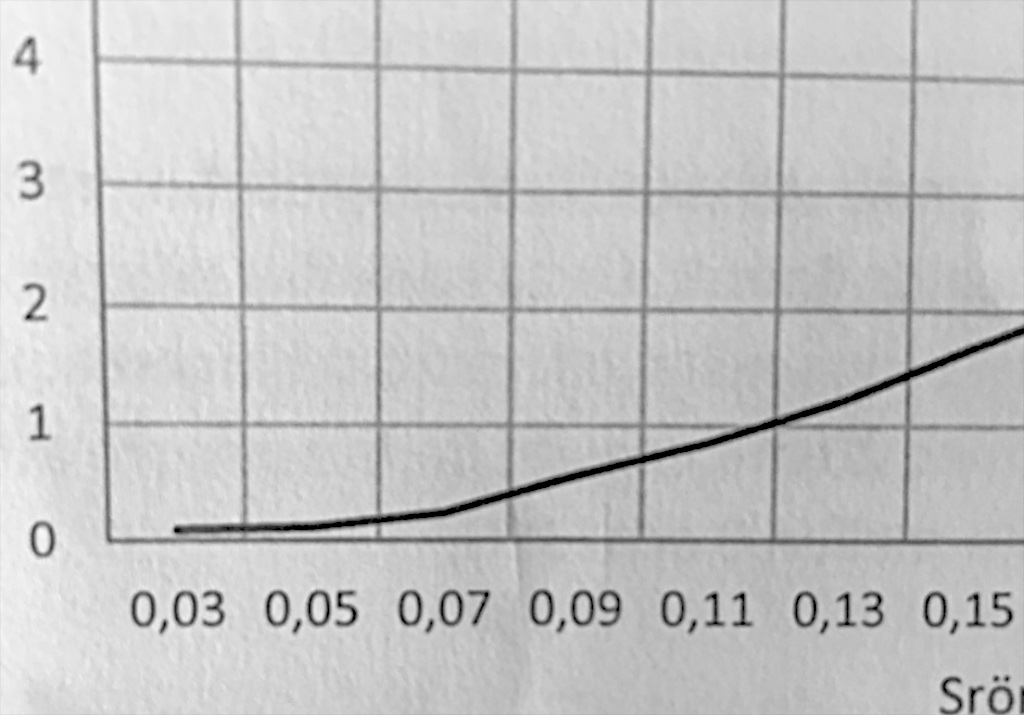
\includegraphics[scale=.2]{skiss.jpg}
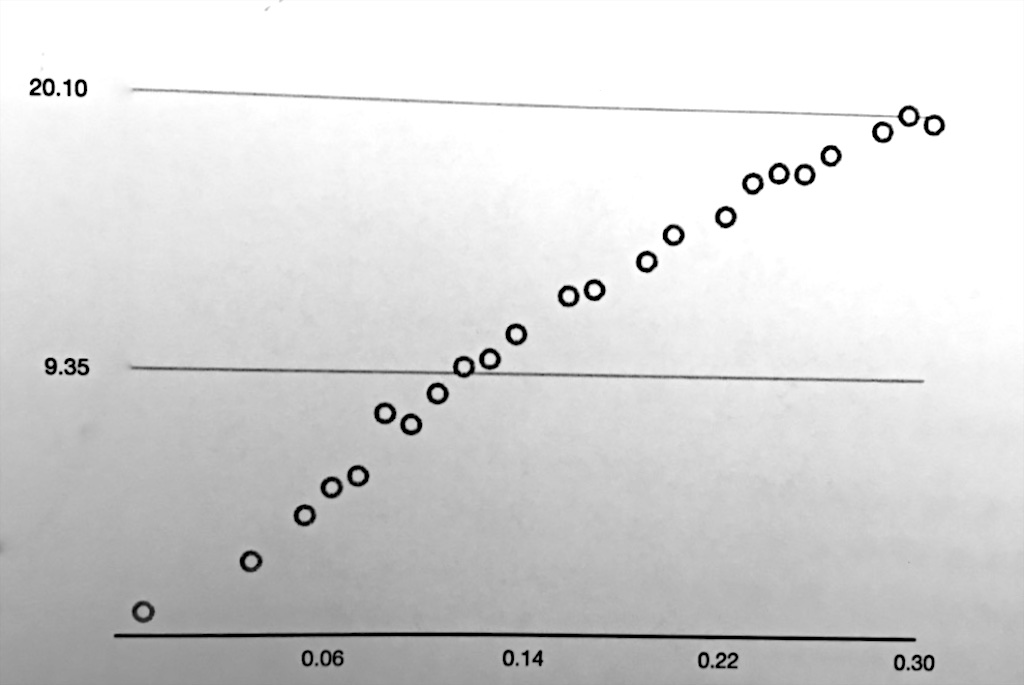
\includegraphics[scale=.2]{skiss1.jpg}
\end{center}

\begin{quote}
\emph{I den vänstra. $x$-axeln: Var är origo? Var är skalstrecken för de angivna värdena? Vad betyder de skalstreck som faktiskt är ditritade? Var är 0.1? $y$-axeln är OK.}

\emph{I den högra. $x$-axeln: Var är origo? Var är skalstrecken för de angivna värdena? Vad ÄR det för värden egentligen? Vad är det för avstånd mellan värdena? $y$-axeln: Var är origo? Var är 5, 10, 20?}
\end{quote}

Ett exempel till: 

\begin{center}
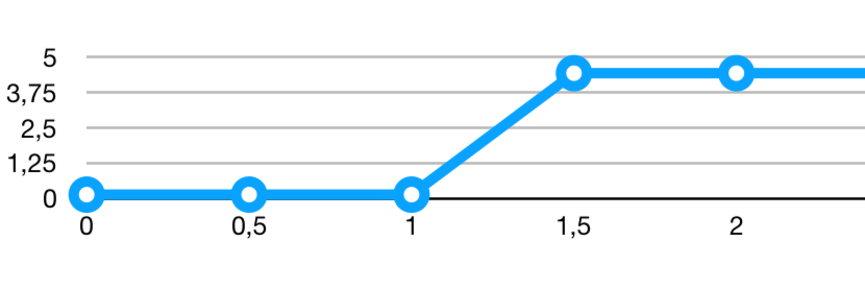
\includegraphics[scale=.7]{skiss3.pdf}
\end{center}

\begin{quote}
\emph{Figuren visar in- och utspänningar i ett 5 voltssystem. Flera problem återfinns: De stora ringarna döljer kurvan här och där. Det är kraftig skillnad mellan en volt i $x$- respektive $y$-led. Här ser man hur $y$-axeln saknas helt. Dessutom är skalan i $y$-led är fel. Inspänningen var upp till 5 V men bara hälften är redovisat. Diagrammet är dessutom så långsmalt att det är svårt att mäta upp något alls i det.}
\end{quote}

Ett försök till: 

\begin{center}
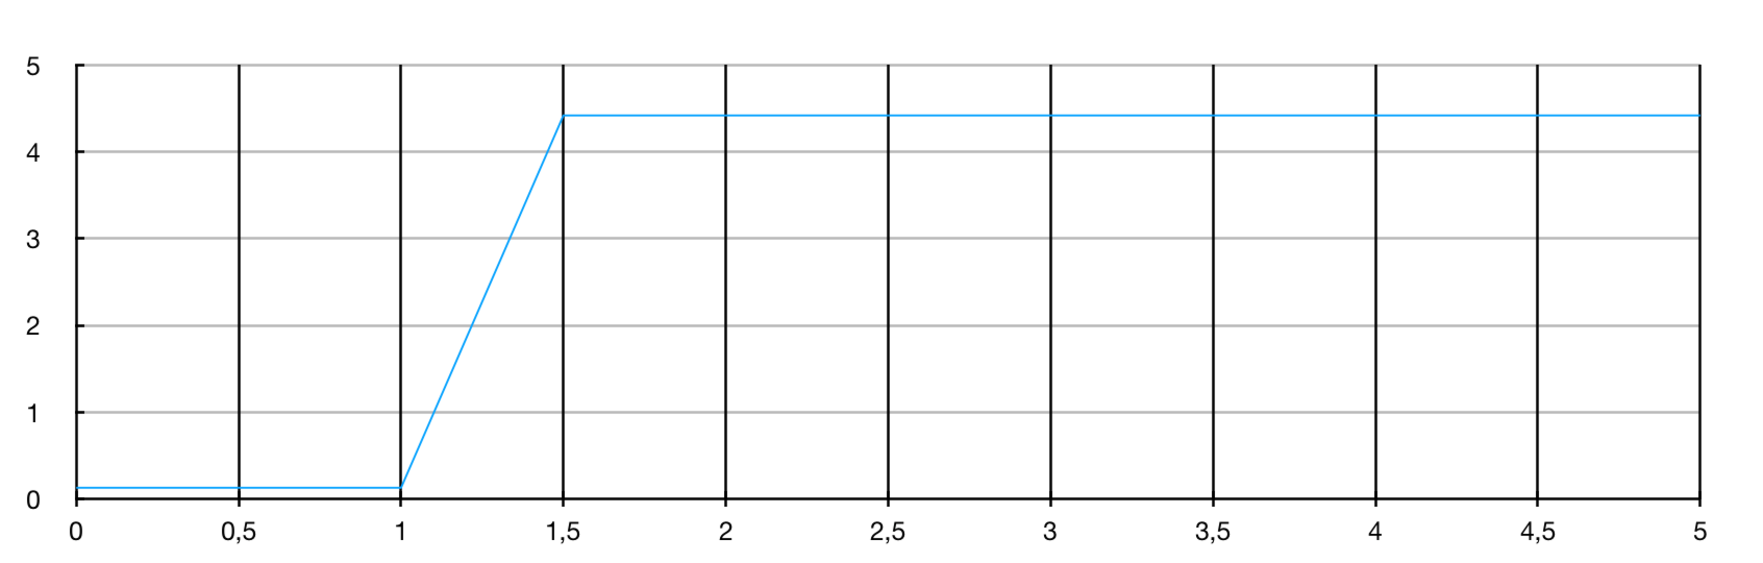
\includegraphics[scale=.5]{skiss2.pdf}
\end{center}


\begin{quote}
\emph{Utan att ändra i indata var det detta som programmet lyckades ta fram som \textsf{2D line}-diagram. Det kan fungera men vackert är det inte.}
\end{quote}

\begin{center}
\begin{tikzpicture}[y=1 cm, x=2 cm]

  % Axis
  \draw [->](0,0)--(0,5.20)node[above right]{$U_u$ [V]};
  \draw [->](0,0)--(5.2,0)node[right]{$U_i$ [V]};

  % Coordinates
  \foreach \x in {0,1,2,3,4,5}
  \draw (\x, 0pt) -- (\x, 0pt) node[anchor=north] {\small{$\x$}};
  \foreach \y in {0,1,2,3,4,5}
  \draw (0pt, \y) -- (0pt, \y) node[anchor=east] {\small{$\y$}};

  % Grid
  \foreach \x in {1,2,3,4,5}
  \draw[dotted] (\x, 0) -- (\x, 5);
  \foreach \y in {1,2,3,4,5}
  \draw[dotted] (0, \y) -- (5, \y);
  
  \foreach \x in {0,1,2,3,4,5}
  \draw[-] (\x, -0.1) -- (\x, 0.1);
    \foreach \x in {0.5,1.5,2.5,3.5,4.5}
  \draw[-] (\x, 0) -- (\x, 0.1);

  \foreach \y in {1,2,3,4,5}
  \draw[-] (-0.05, \y) -- (0.05, \y);

  % Functions
  \draw plot[mark=., mark options={fill=black}]
      file {exdata.dat};

\end{tikzpicture} 
\end{center}

\begin{quote}
\emph{Samma mätdata men i ett bättre diagram. Diagrammet har renare linjer som inte stör kurvan och ändamålsenliga skalmarkeringar. Antalet mätpunkter är för få för i det intressanta området där någonting händer.}
\end{quote}

\section*{Logaritmiska diagram}

Bland det vanligaste olineära diagram för tekniska tillämpningar inom elektronik, reglerteknik, signalbehandling, filterteori osv återfinns det \emph{logaritmiska} 
diagrammet. 

Om enbart $x$-axeln är logaritmisk kallas det \emph{linlog}-diagram då $y$-axeln fortfarande är lineär. Linlog-diagrammet nedan täcker hela tre \emph{dekader}\footnote{En dekad utgör en kvot av tio.} längs $x$-axeln, exempelvis frekvensområdet 10--100--1000 Hz.

 
\begin{center}
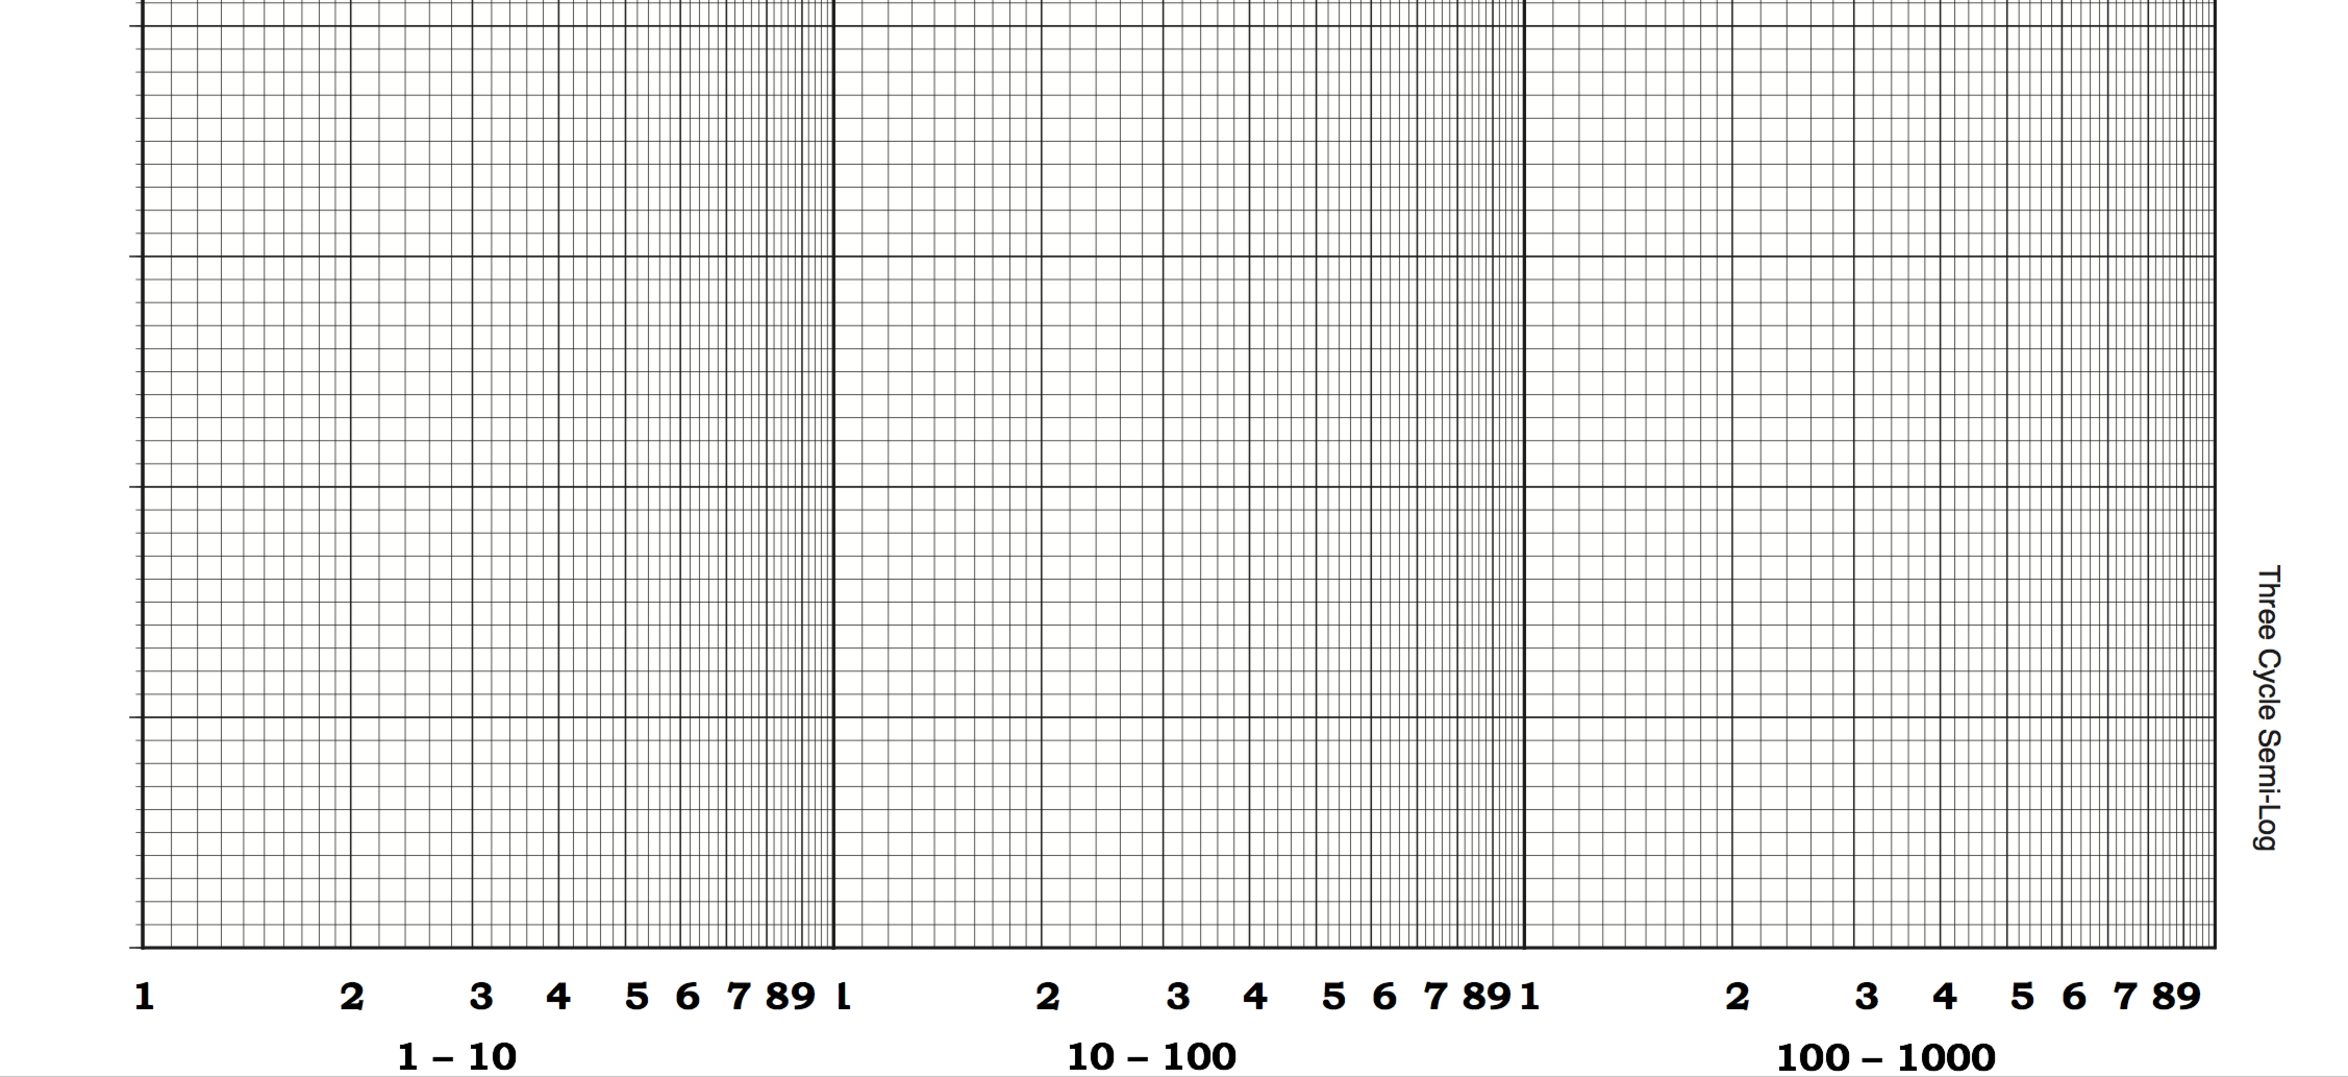
\includegraphics[scale=0.4]{linlog-skala.pdf}
\end{center}

Då $x$-skalan är logaritmerad kommer exponentialfunktioner att ritas som räta linjer. Man kan lätt tillverka sin egen logaritmerade skala genom logaritmen på skalvärdet (något förstorad för att få värden i millimeter):

\begin{multicols}{2}
\begin{tabular}{ccr}
$x$ & $\log x$ & $100\cdot \log x$ (mm)\\
\hline
1 & 0.000 & 0\\
2& 0.301 & 30\\
3& 0.477 & 48\\
4& 0.602 & 60\\
5& 0.699 & 70\\
6& 0.778 & 78\\
7& 0.845 & 85\\
8& 0.903 & 90\\
9& 0.954 & 95\\
10& 1.000 & 100\\
\end{tabular}

Man ser att de logaritmerade värdena blir tätare och tätare  längre ner i tabellen. Detta motsvaras av att skalindelningen blir tätare i linlog-diagrammet ovan.

Man kan notera att det är \emph{ungefär} samma avstånd  1--2 som  2--5 och som  5--10. På ett ungefär kan man dela upp dekaden i tredjedelar och få ett hyggligt logaritmisk skala på det sättet.

\end{multicols}

\newpage

\subsection*{Loglogplot av $\frac{1}{x^2}$}

\begin{multicols}{2}

Funktionen \[ F(x)=\frac{1}{x^2} \hspace{7mm} x\in {0.1\ldots50}\] önskas plottad i ett log-logdiagram.\footnote{Med $F(x)$ logaritmerad som $\log F(x) = 0 - \log{x^2}=-2 \log {x}$ bör den resulterande linjen i ett diagram, med båda axlarna logaritmerade, bli en rät linje med en viss lutning.}

Om mätvärdena utgör amplitudvärden beräknas decibeltalet som $20 \log F(x)$, om det är effektvärden beräknas de  enligt $10 \log F(x)$.

En värdetabell över funktionen och dess logaritm uttryckt i decibel (spänningsförstärkning antages) blir: 

\begin{tabular}{rrr}
$x$ & $F(x)$ & $20 \log F(x)$\\
\hline
0.1  & 100   & 40 \\
0.2  &25     & 28 \\ 
0.5  &4      & 12 \\
1    &1      & 0 \\
2    &0.25   & --12 \\
5    &0.04   & --28  \\
10   &0.01   & --40  \\
20   &0.0025  & --51 \\
50   &0.0004  & --68 \\
\end{tabular}

\end{multicols}

\begin{center}
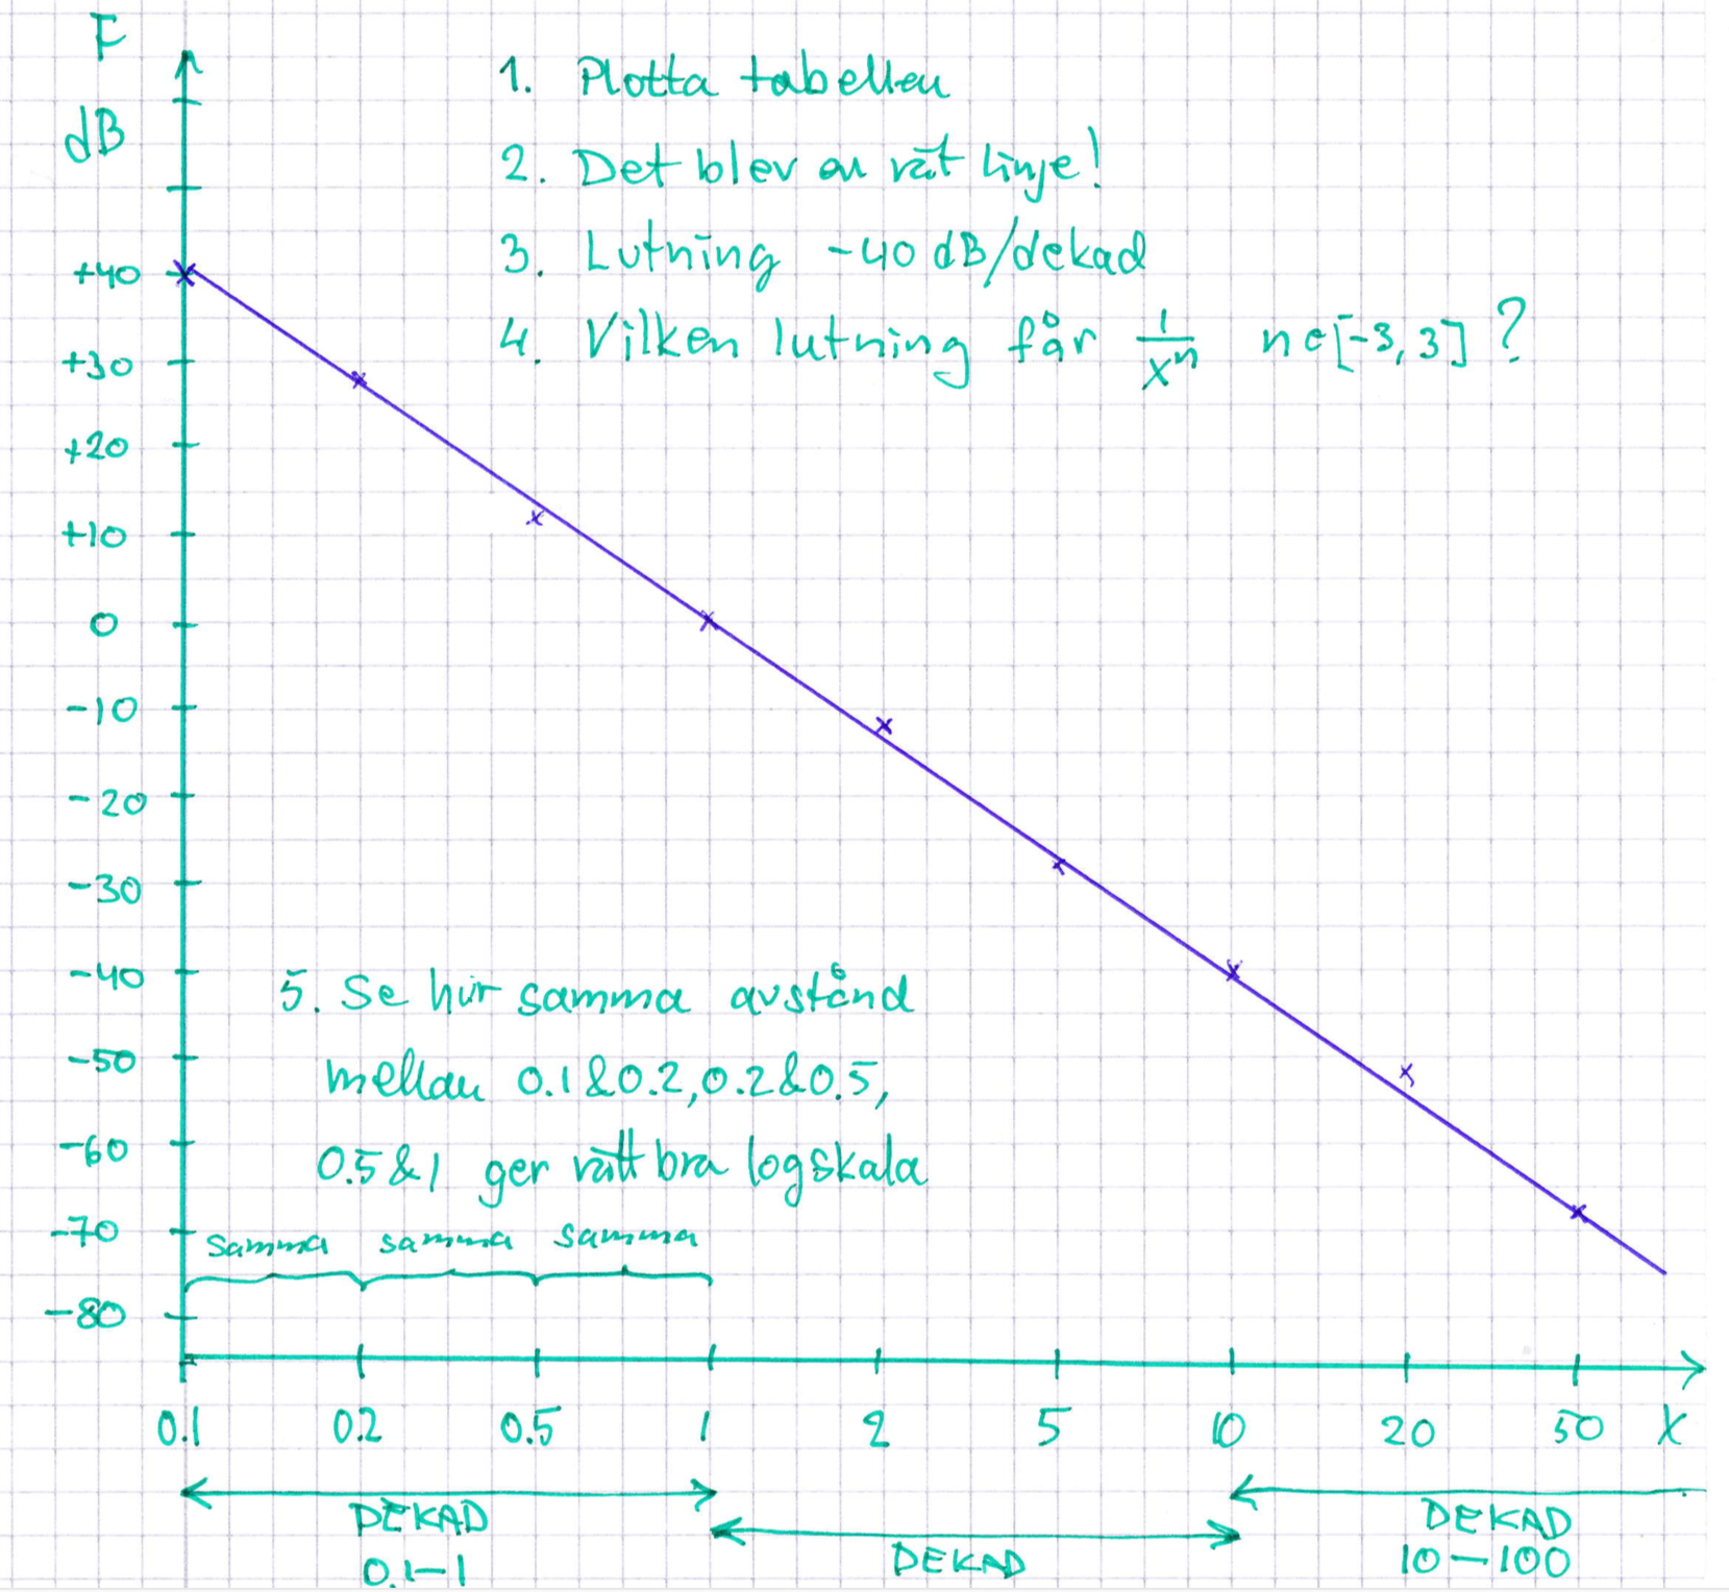
\includegraphics[scale=0.5]{linlog.pdf}
\end{center}

I figuren ser man att det \emph{dels} blev en rät linje som förutspått  och \emph{dels} att en ''nästan-logskala'' snabbt kan tillverkas kan genom att dela en dekad i tredjedelar.

%För att visa frekvensgången (förstärkning som funktion av frekvensen) hos, till exempel, en förstärkare  utgörs $y$-axeln av en decibel-skala varför man själv får beräkna dB-värdet innan det förs in på den lineära $y$-axeln. Själva $y$-axeln har alltså samma avstånd mellan varje dB, men värdena är logaritmerade.

\subsubsection*{Uppgift}

%För att bekanta dig med diagramtyperna kan du prova enligt punkterna nedan. 

Rita \emph{för hand}. Ja, för hand. Det är som vi sett svårt att tvinga ur de vanligaste kalkylprogrammen ett  acceptabelt tekniskt diagram. Försök inte ens. Bestäm dig först för hur diagrammet skall se ut, rita det sedan så! Tänk över skalorna, skalindelning och slutligt resultat.

\begin{multicols}{2}
\begin{enumerate}

\item Följande värden på svängningstid för en pendel upphängd i ett masslöst snöre uppmättes. Tabellen anger tid i sekunder, tagen som medelvärde över 20 svängningar, som funktion av längd på snöret.

\begin{tabular}{cc}
Längd (cm) & Tid (s)\\
\hline
233   & 3.071 \\
194   & 2.791 \\ 
171   & 2.634 \\
158   & 2.545 \\
141   & 2.397 \\ 
116   & 2.175 \\ 
90    & 1.926 \\
68    & 1.702 \\
52    & 1.451 \\
\hline
\end{tabular}

\vspace{2cm}

\begin{enumerate}
\item Rita diagram över \emph{längd som funktion av tid}, $L(T)$. Sätt lämpliga lineära skalor.
\item Det finns anledning att anta att sambandet är av typen \[ T(L)=C\cdot L^k \] Logaritmering av båda sidor ger \[ \log T = \log C + k\cdot\log L  \] Om antagandet är korrekt motsvarar detta en rät linje i ett log-log-diagram. Rita sambandet $T$ som funktion av $L$ i ett lämpligt diagram med logaritmiska skalor på båda axlarna. 
\end{enumerate}

%\item  Rita grafen för $f(x)=x^2$ respektive $f(x)=x^3$  och deras logaritmer i ett diagram med lineär $x$-skala. $x=0.01-10$.

%\item Rita grafen för $f(x)=x^2$ respektive $f(x)=x^3$  och deras logaritmer i ett diagram med logaritmisk $x$-skala. $x=0.01-10$. 

%\item [3] Rita beloppet av reaktansen som funktion av frekvensen för $X(\omega)=\frac{1}{j\omega C}$. Antag $C=18$ $\mu$F. Prova i både lineär och logaritmisk skala. Vilken blir snyggast? ($\omega$ är vinkelfrekvens i rad/s. $\omega = 2\pi f$ om frekvens önskas i Hz.
%\item [4] Som ovan fast för $f(\omega)=\frac{1}{\omega ^2 - 5}$. 

%\item [5] Rita beloppet som funktion av frekvens för $f(\omega)=j \omega L$. Antag L=10 mH.
%\item [5] Rita beloppet $|Z|=\sqrt{R^2+(\omega L - \frac{1}{\omega C})^2}$ som funktion av frekvensen $f$ och som funktion av vinkelfrekvensen $\omega=2 \pi f$ då  L=10 mH, C=18 $\mu$F, R=15 $\Omega$. 
\end{enumerate}

\end{multicols}





\begin{center}\textbf{Visar diagrammet verkligen det du vill ha fram?}\end{center}

\begin{center}

o-x=Ö=x-o
\end{center}


\hspace{-20mm}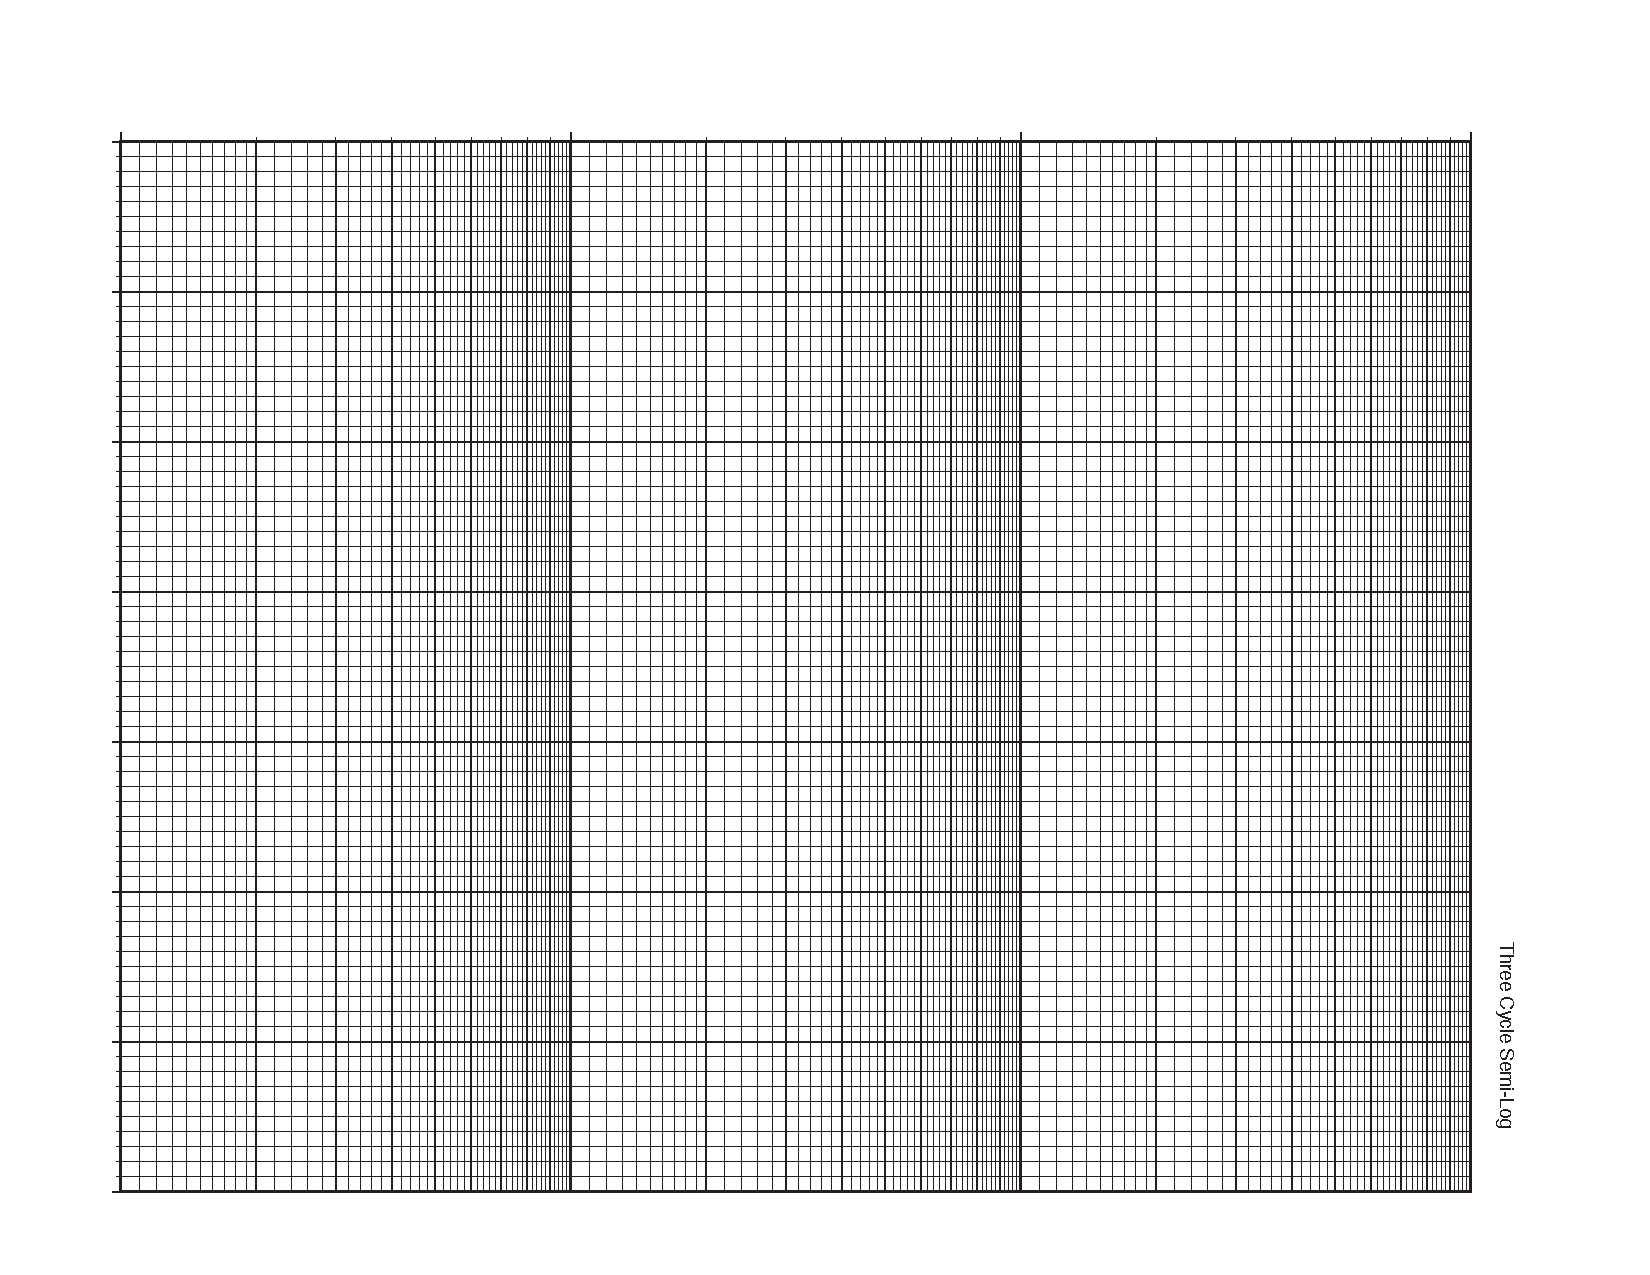
\includegraphics[angle=90,scale=0.85]{linlog-papper.pdf}

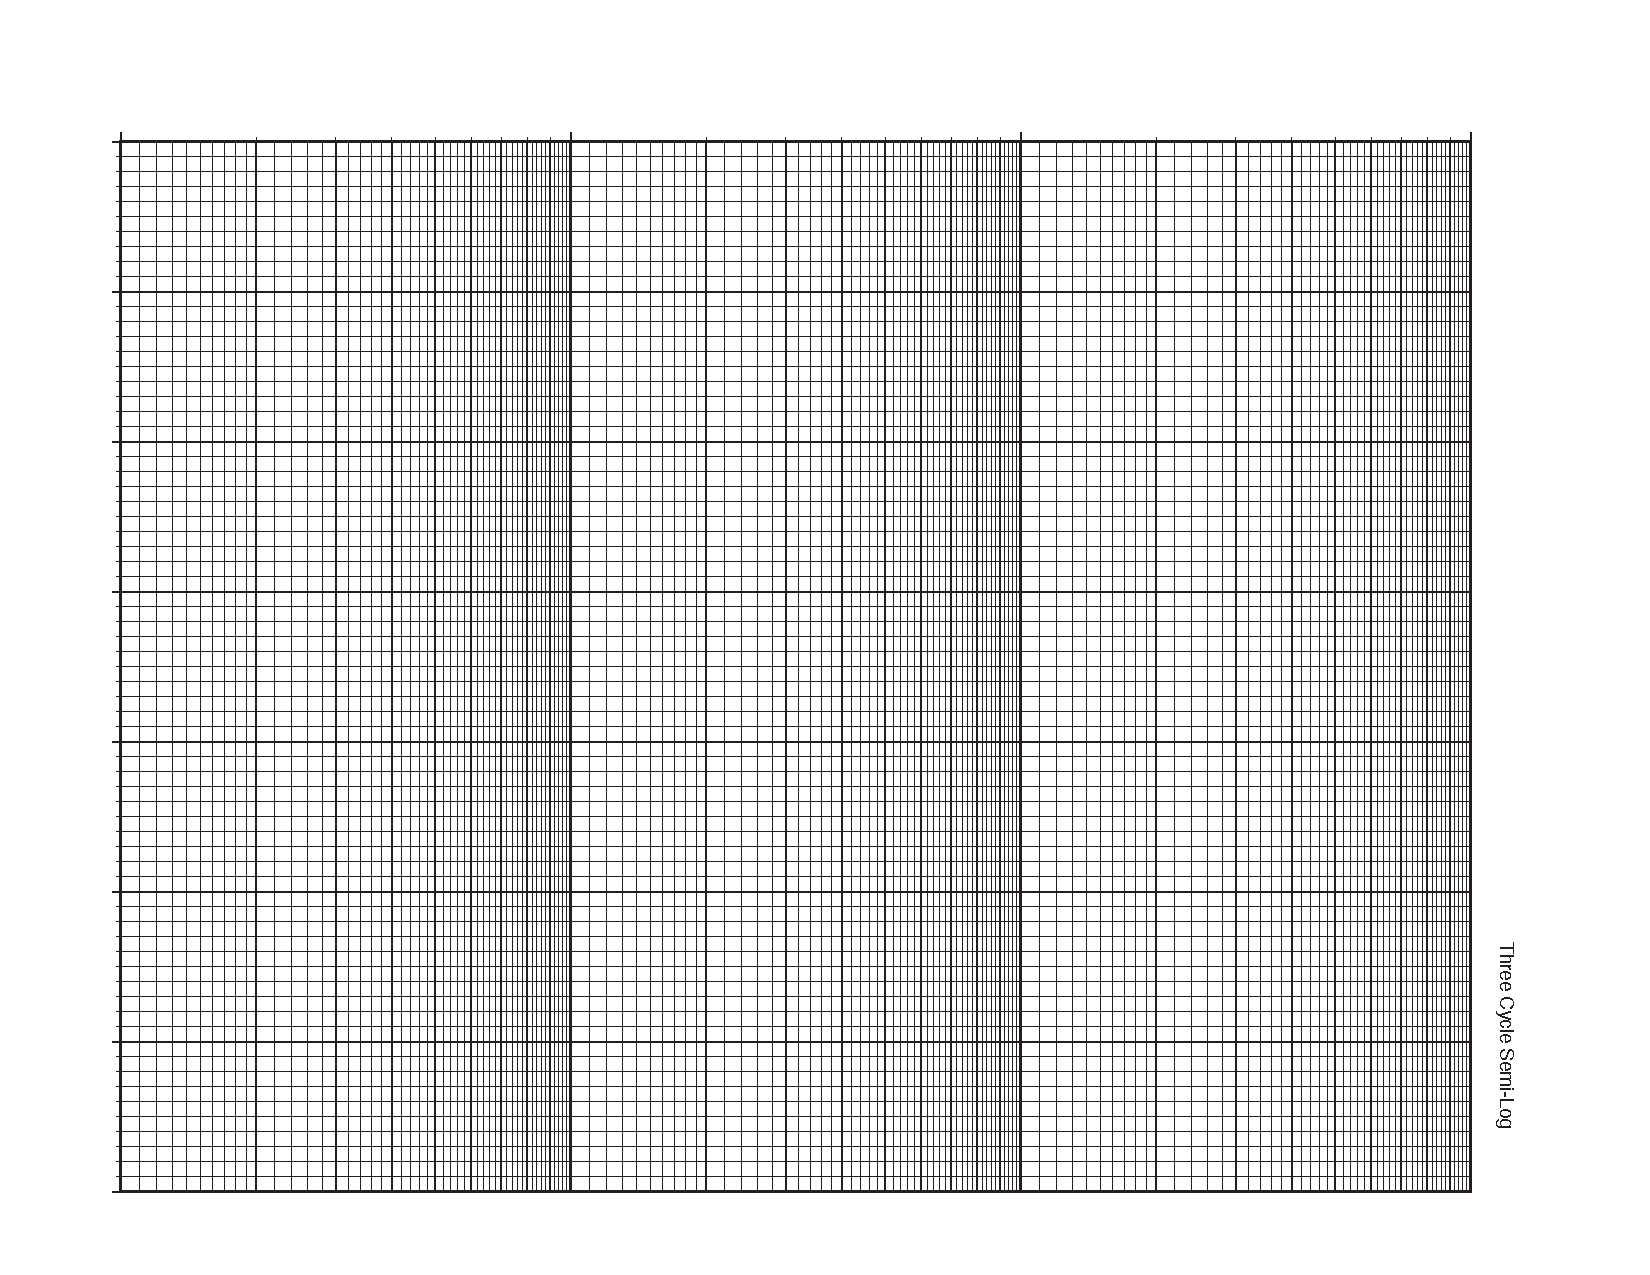
\includegraphics[angle=90,scale=0.85]{linlog-papper.pdf}

\hspace{-20mm}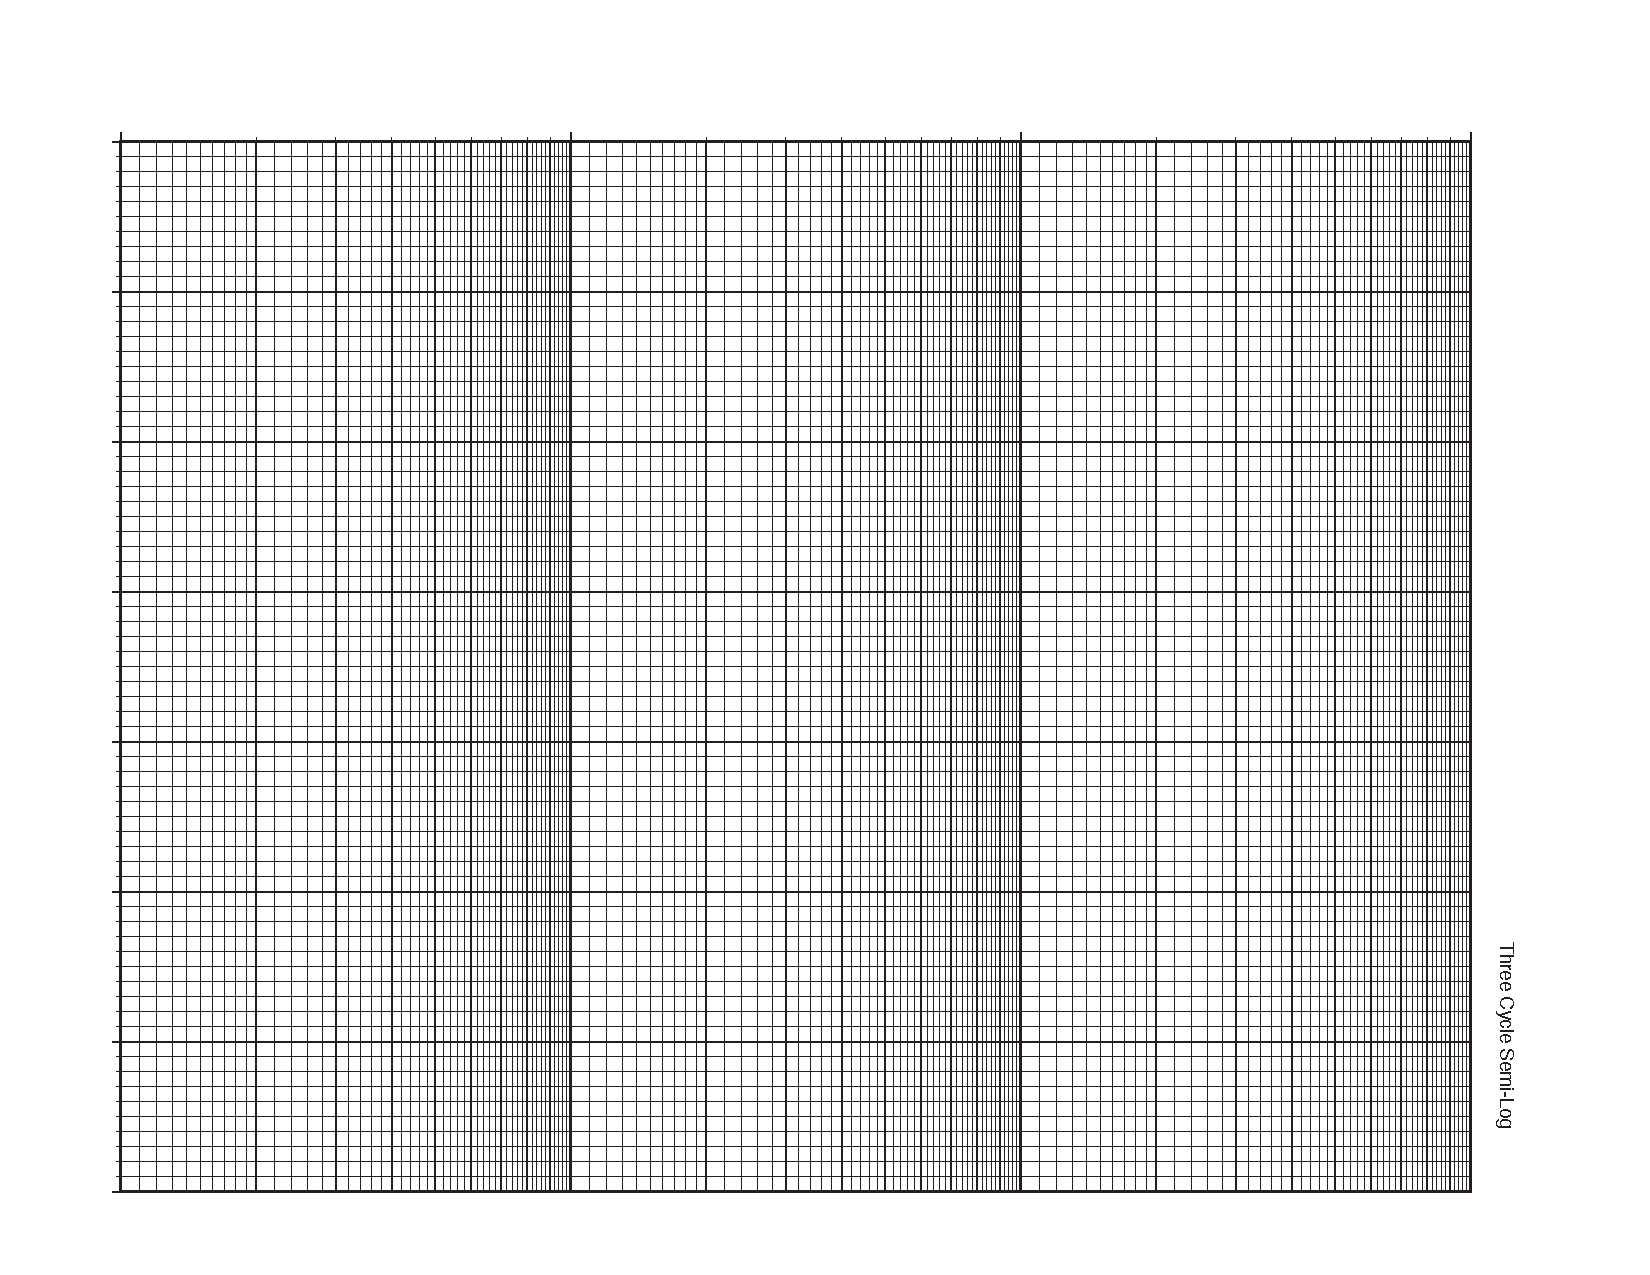
\includegraphics[angle=90,scale=0.85]{linlog-papper.pdf}



\end{document}